% -- Generated using the code: moving_clocks_single_fig(-0.3, 0.3, -1.5, 5, -1)



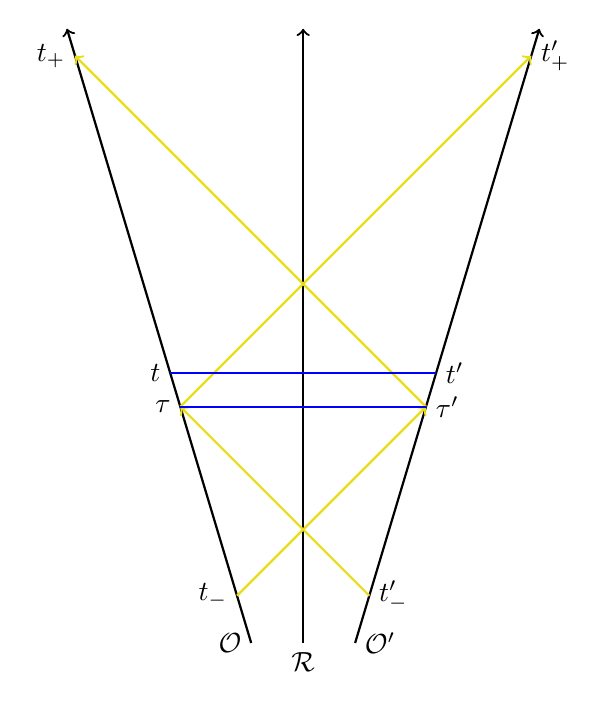
\begin{tikzpicture}[scale=1.2]
	% Draw lines of observers
	\draw[->, thick] (-0.55, -1.5) -- (-2.5, 5);
	\draw[->, thick] (0.55, -1.5) -- (2.5, 5);
	\draw[->, thick] (-0.0, -1.5) -- (0.0, 5);
	
	% Draw trajectories of light
	\draw[->, thick, black!10!yellow] (-0.7, -1) -- (1.3, 1.0);
	\draw[->, thick, black!10!yellow] (1.3, 1.0) -- (-2.4142857142857137, 4.7142857142857135);
	\draw[->, thick, black!10!yellow] (0.7, -1.0) -- (-1.3, 1.0);
	\draw[->, thick, black!10!yellow] (-1.3, 1.0) -- (2.4142857142857137, 4.7142857142857135);
	
	% Draw lines of simultaneity
	\draw[thick, blue] (-1.407142857142857, 1.357142857142857) -- (1.407142857142857, 1.357142857142857);
	%\draw[thick, blue] (-1.557142857142857, 1.8571428571428568) -- (1.557142857142857, 1.8571428571428568);
	\draw[thick, blue] (-1.3, 1.0) -- (1.3, 1.0);
	
	% Make labels
	\draw (-0.55, -1.5) node[left] {$\mathcal{O}$};
	\draw (-0.7, -1) node[left] {$t_-$};
	\draw (-2.4142857142857137, 4.7142857142857135) node[left] {$t_+$};
	\draw (1.3, 1.0) node[right] {$\tau'$};
	\draw (1.407142857142857, 1.357142857142857) node[right] {$t'$};
	%\draw (1.557142857142857, 1.8571428571428568) node[right] {$t'$};
	\draw (0.55, -1.5) node[right] {$\mathcal{O}'$};
	\draw (0.7, -1.0) node[right] {$t'_-$};
	\draw (2.4142857142857137, 4.7142857142857135) node[right] {$t'_+$};
	\draw (-1.3, 1.0) node[left] {$\tau$};
	\draw (-1.407142857142857, 1.357142857142857) node[left] {$t$};
	%\draw (-1.557142857142857, 1.8571428571428568) node[left] {$t$};
	\draw (-0.0, -1.5) node[below] {$\mathcal{R}$};
\end{tikzpicture}